\documentclass{beamer}
\usepackage{graphicx}
\usepackage{hyperref}

\usetheme[subsectionpage=progressbar]{metropolis}

\title{On Being a Research Computer Scientist}
\subtitle{or what it's like to be a lifelong learner}
\date{November 15\textsuperscript{th}, 2018}
\author{Anthony J. Christe}
\institute{University of Hawaii at Manoa \\ Slippery Rock University of Pennsylvania}

\begin{document}
\maketitle

\section{Introduction}
\begin{frame}{What People Think I Do}
\begin{figure}
	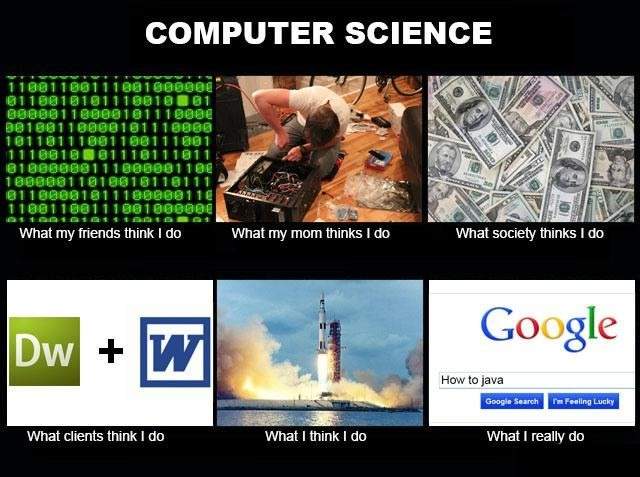
\includegraphics[width=\linewidth]{img/whatido.jpg}
\end{figure}
\end{frame}

\begin{frame}{What I actually do}
\begin{itemize}
	\item Working to obtain PhD in Computer Science
	\begin{itemize}
		\item With an emphasis on Big Data
		\item Distributed sensor networks
		\item Distributed computing
	\end{itemize}
	\item Research Assistant for Infrasound Laboratory
	\begin{itemize}
		\item Design and develop systems for capture, analysis, and reporting of infrasonic signals of interest
	\end{itemize}
\end{itemize}
\end{frame}

\section{How I Got Here}
\begin{frame}{Summary of My Life Until Now}
\begin{itemize}
	\item Graduated High School
	\begin{itemize}
		\item Somerset, PA 2007
	\end{itemize}
	\item B.S. in Computer Science (w/ minor in Theatre)
	\begin{itemize}
		\item Slippery Rock University of PA, 2011
	\end{itemize}
	\item M.S. in Computer Science
	\begin{itemize}
		\item University of Hawaii at Manoa, 2015
	\end{itemize}
	\item Ph.D. in Computer Science
	\begin{itemize}
		\item University of Hawaii at Manoa, Present
	\end{itemize}
\end{itemize}
\end{frame}

\subsection{High School}
\begin{frame}{High School}
\begin{itemize}
	\item No Formal Education in Computer Science
	\item Some self taught Python
	\item Web technologies for cool AIM profiles
	\item Band Geek
	\item Theatre Geek
\end{itemize}
\end{frame}

\subsection{Undergraduate Education}
\begin{frame}{Slippery Rock University of Pennsylvania}
	\begin{columns}
		\begin{column}{.34\textwidth}
			\begin{itemize}
				\item Small class sizes
				\item \emph{Close} to home
				\item Ski slope
				\item State school
			\end{itemize}
		\end{column}
		\begin{column}{.66\textwidth}
			\begin{figure}
				
\includegraphics[width=\linewidth]{img/sru.jpg}
			\end{figure}
		\end{column}
	\end{columns}
\end{frame}

\begin{frame}{Slippery Rock University of Pennsylvania}
\begin{figure}
	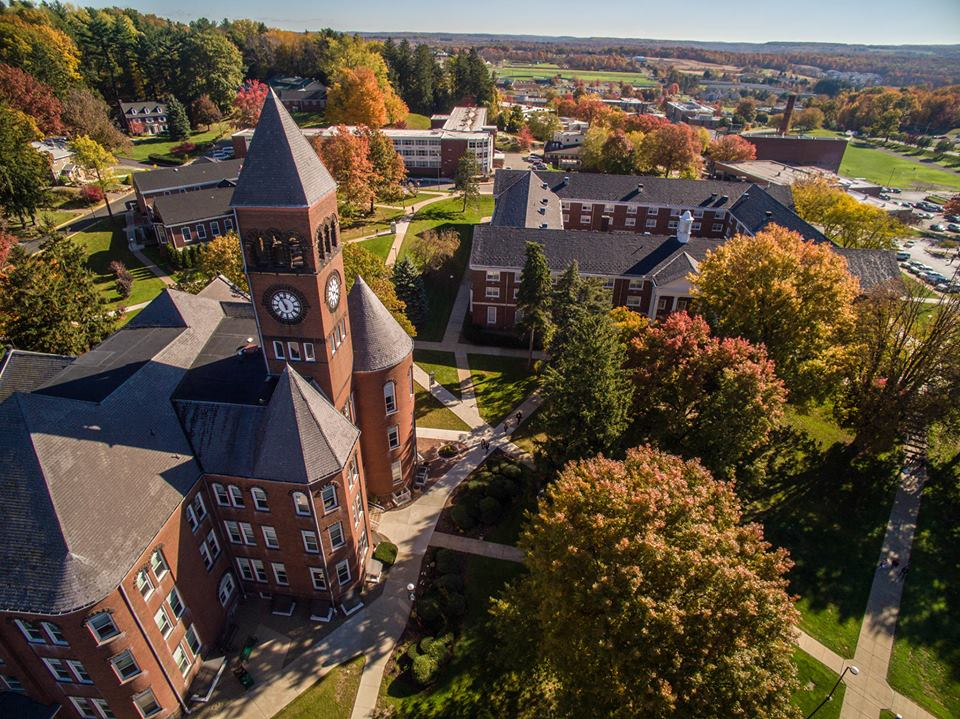
\includegraphics[width=\linewidth]{img/sru2.jpg}
\end{figure}
\end{frame}

\begin{frame}{Slippery Rock University of Pennsylvania}
\begin{figure}
	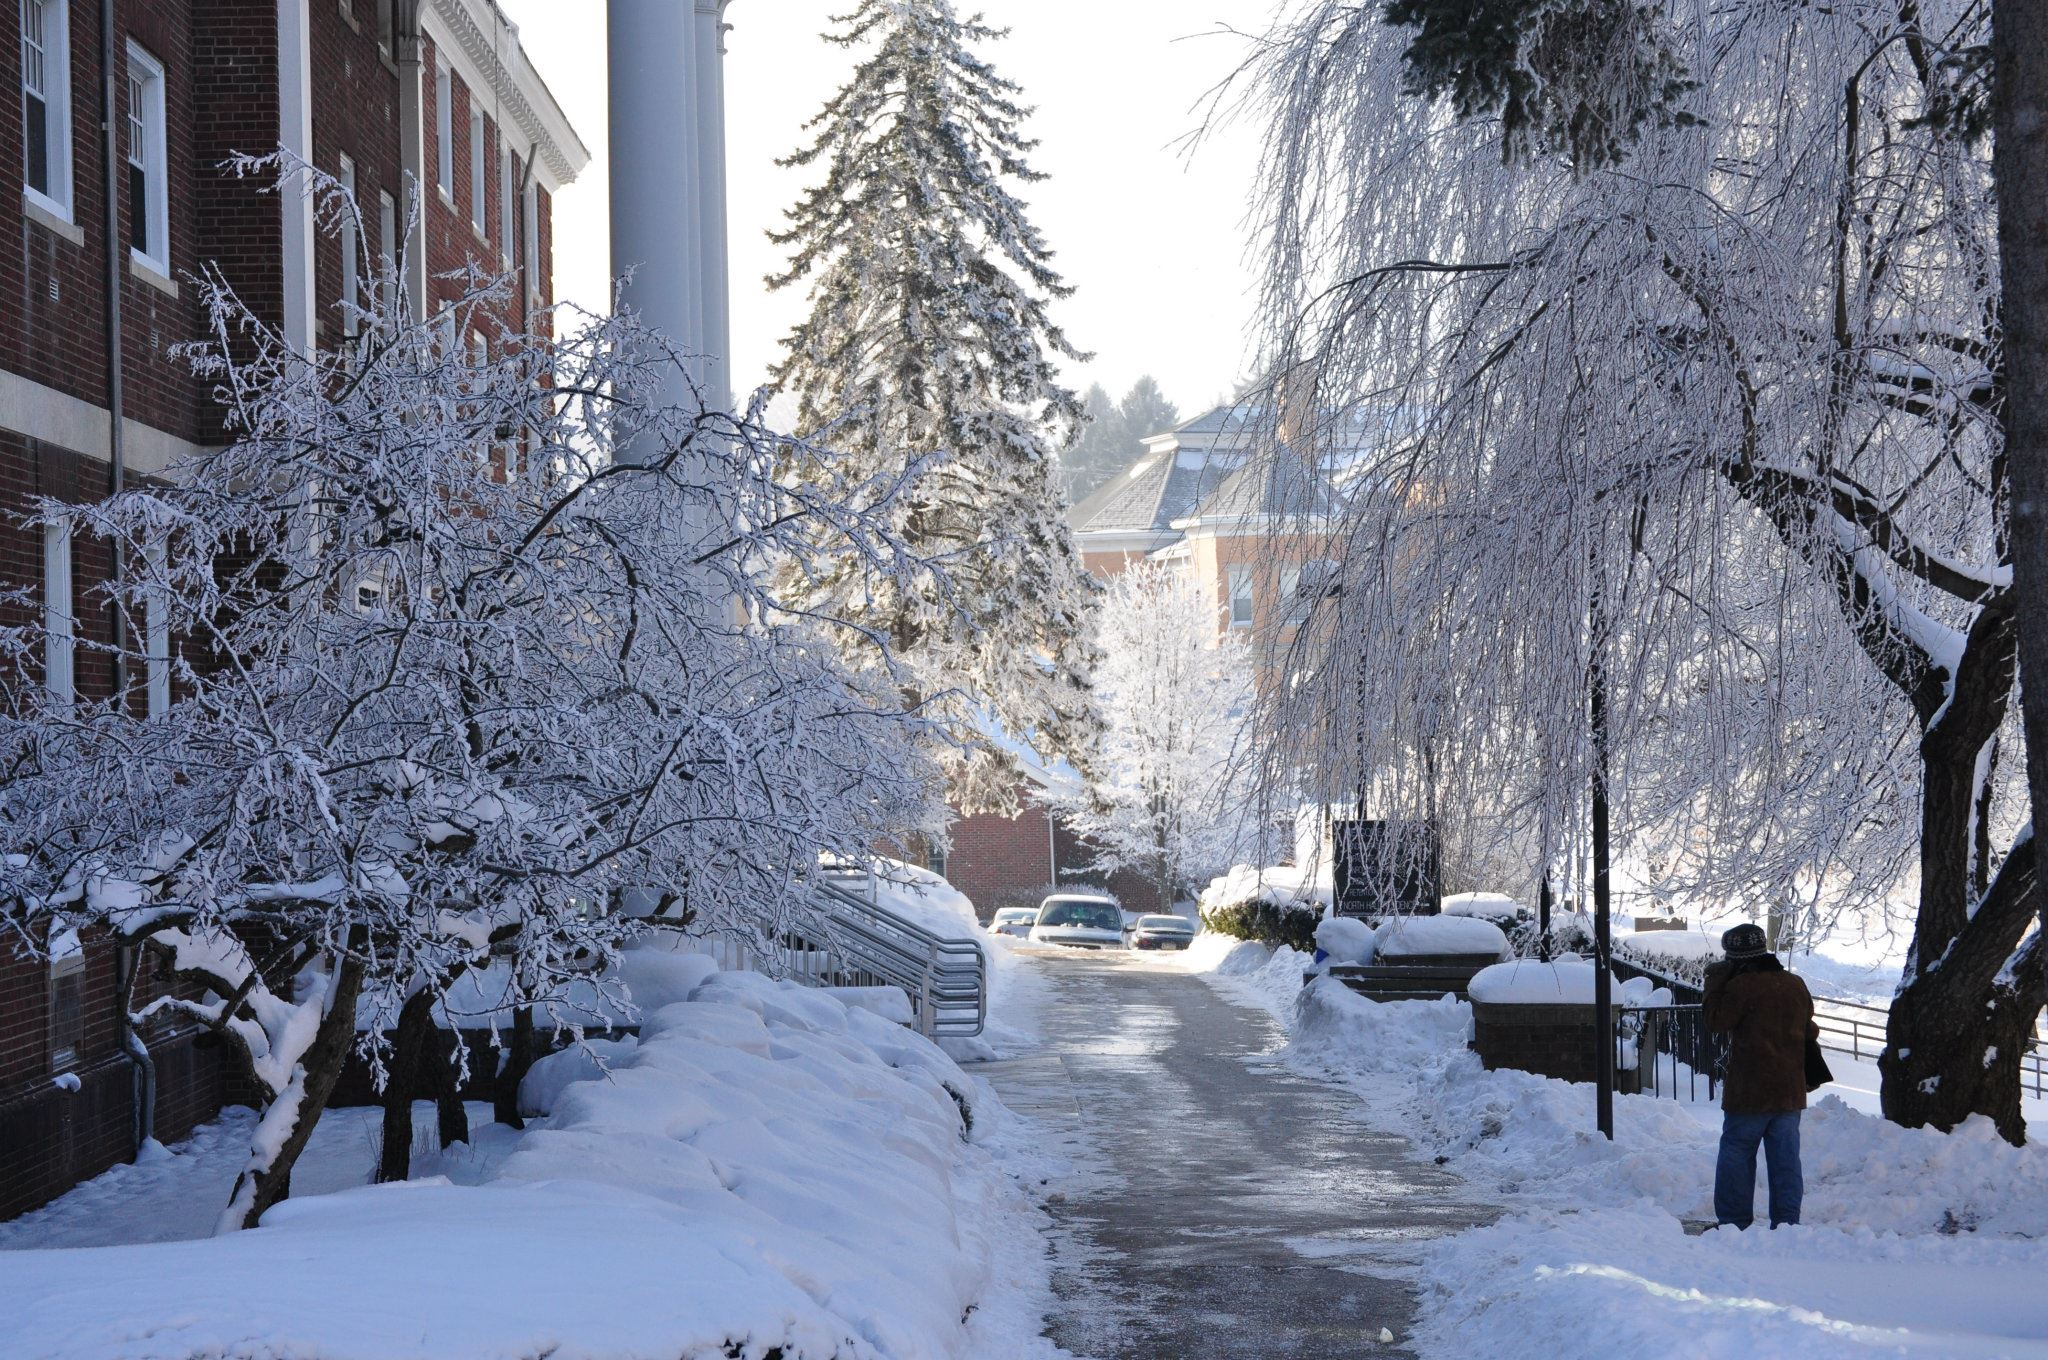
\includegraphics[width=\linewidth]{img/sru4.jpg}
\end{figure}
\end{frame}

\begin{frame}{Slippery Rock University of Pennsylvania}
\begin{figure}
	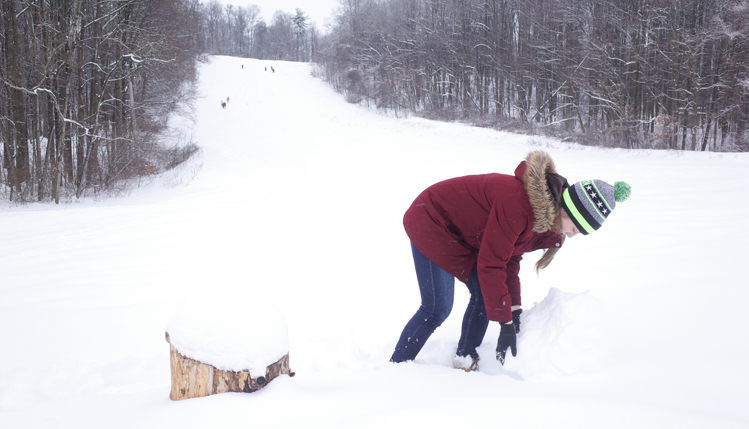
\includegraphics[width=\linewidth]{img/sru3.jpg}
\end{figure}
\end{frame}

\begin{frame}{Computer Science is \emph{not}} 
\centering 
\includegraphics[width=.5\linewidth]{img/fortnite.jpg}
\end{frame}

\begin{frame}{Undergraduate Computer Science}
\begin{itemize}
	\item Computer Science \emph{is}
	\begin{itemize}
		\item Algorithms
		\item Data structures
		\item Software Engineering
		\item Operating Systems
		\item Artificial Intelligence
		\item Mathematical
		\item ...
		\item \emph{Social}
	\end{itemize}
\end{itemize}
\end{frame}

\begin{frame}
\begin{figure}
	
\includegraphics[width=\linewidth]{img/all_the_things.jpg}
\end{figure}
\end{frame}

\begin{frame}{Artificial Intelligence Robot}
\begin{itemize}
	\item Used genetic algorithms to \emph{teach} a robot to pick up a ball
	\item Machine vision/image processing utilized to find the ball
	\item Wrote a script interpreter
	\begin{itemize}
		\item Programming language for the robot
		\item Could perform movements in parallel
	\end{itemize}
	\item \url{https://www.youtube.com/watch?v=xoBVfaHHHcI}
\end{itemize}
\begin{figure}
	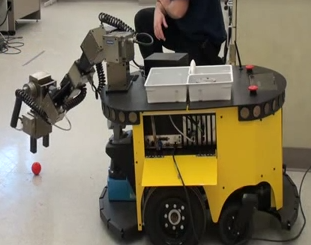
\includegraphics[width=.45\linewidth]{img/robot.png}
\end{figure}
\end{frame}

\begin{frame}{Boulders Computer Cluster}
\begin{itemize}
	\item Used 8 recycled Intel blade servers to build a computer cluster
	\item A single master server managed all slave nodes
	\item Operating system loaded on each slave via PXE
	\item HPC via message passing interface (MPI)
	\begin{itemize}
		\item MapReduce
		\item Apache Spark
		\item \emph{...and many more...}
	\end{itemize}
\end{itemize}
\end{frame}

\begin{frame}{Other Undergrad Activities}
\begin{columns}
	\begin{column}{.50\textwidth}
		\begin{itemize}
			\item Vice-president of $\Upsilon\Pi$E
			\item President of Computer Technology Club
			\item Student Advisor to the Dean
			\item Minor in Theatre
		\end{itemize}
	\end{column}
	\begin{column}{.50\textwidth}
		\begin{figure}
			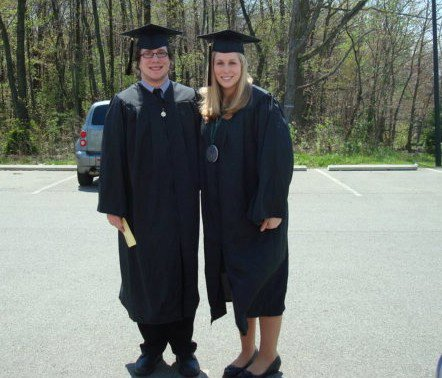
\includegraphics[width=\linewidth]{img/chrissie.jpg}
		\end{figure}
	\end{column}
\end{columns}
\end{frame}

\begin{frame}{After Graduation}
\begin{figure}
	
\includegraphics[width=\linewidth]{img/uh.png}
\end{figure}
\end{frame}

\subsection{Graduate School}

\begin{frame}{What is Graduate School?}
\begin{itemize}
	\item Education beyond your bachelor's degree
	\begin{itemize}
		\item Masters, Ph.D, M.D., Ed.D., \emph{etc}
	\end{itemize}
	\item Generally funded through teaching/research assistantship
	\item Specialization of your field
	\item Research focused
	\item Expects publishing and attending conferences
	\item Novel contribution to the field (Ph.D.)
\end{itemize}
\end{frame}

\begin{frame}{Master's Degree}
	\begin{itemize}
		\item Specialization in your field
		\item Comprehensive project \emph{or}
		\item Master's thesis
		\item Graduate classes
	\end{itemize}
\end{frame}

\begin{frame}{Teaching Assistantship (TA)}
\begin{itemize}
	\item ICS 211 - Intro. to Programming II
	\begin{itemize}
		\item 5 Semesters
		\item Run programming lab
		\item Design homework assignments (sometimes)
		\item Grade homework assignments
		\item Run lecture (when needed)
	\end{itemize}
\end{itemize}
\end{frame}

\begin{frame}{Research Assistantship (RA)}
\begin{itemize}
	\item Paid to perform research 
	\begin{itemize}
		\item Income \textasciitilde\$25,000/yr
		\item Tuition waver \textasciitilde\$22,000/yr
	\end{itemize}
	\item Many more opportunities than a TA
	\item OpenPowerQuality - 1 Semester
	\item Infrasound Laboratory - Current
\end{itemize}
\end{frame}

\begin{frame}{OpenPowerQuality (OPQ)}
	\begin{columns}
		\begin{column}{.50\textwidth}
			\begin{itemize}
				\item Open source distributed sensors and framework
				\begin{itemize}
					\item Detects PQ problems
					\item Stores raw data in cloud
					\item Performs analytics
					\item Reports PQ info to users
				\end{itemize}
			\end{itemize}
		\end{column}
		\begin{column}{.50\textwidth}
			\begin{figure}
				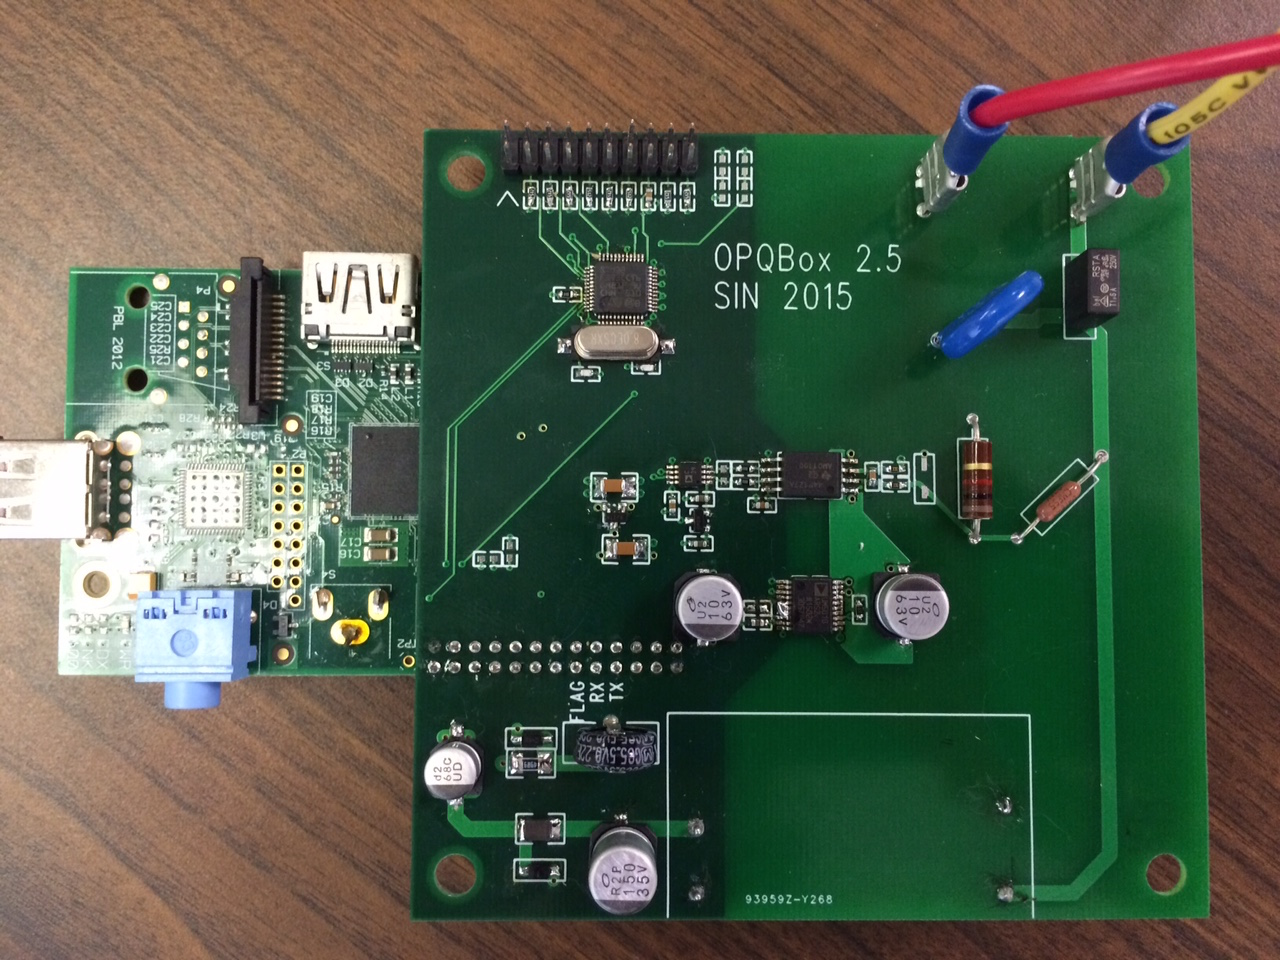
\includegraphics[width=\linewidth]{img/box.jpg}
			\end{figure}
		\end{column}
	\end{columns}
\end{frame}

\begin{frame}{Infrasound Laboratory}
\begin{columns}
	\begin{column}{.60\textwidth}
		\begin{itemize}
			\item Sound <20 Hz
			\item Generated by large movements of air
			\begin{itemize}
				\item Volcanoes
				\item Explosions
				\item Storms
				\item Aircraft
				\item Rockets
			\end{itemize}
		\end{itemize}
	\end{column}
	\begin{column}{.40\textwidth}
		\begin{figure}
			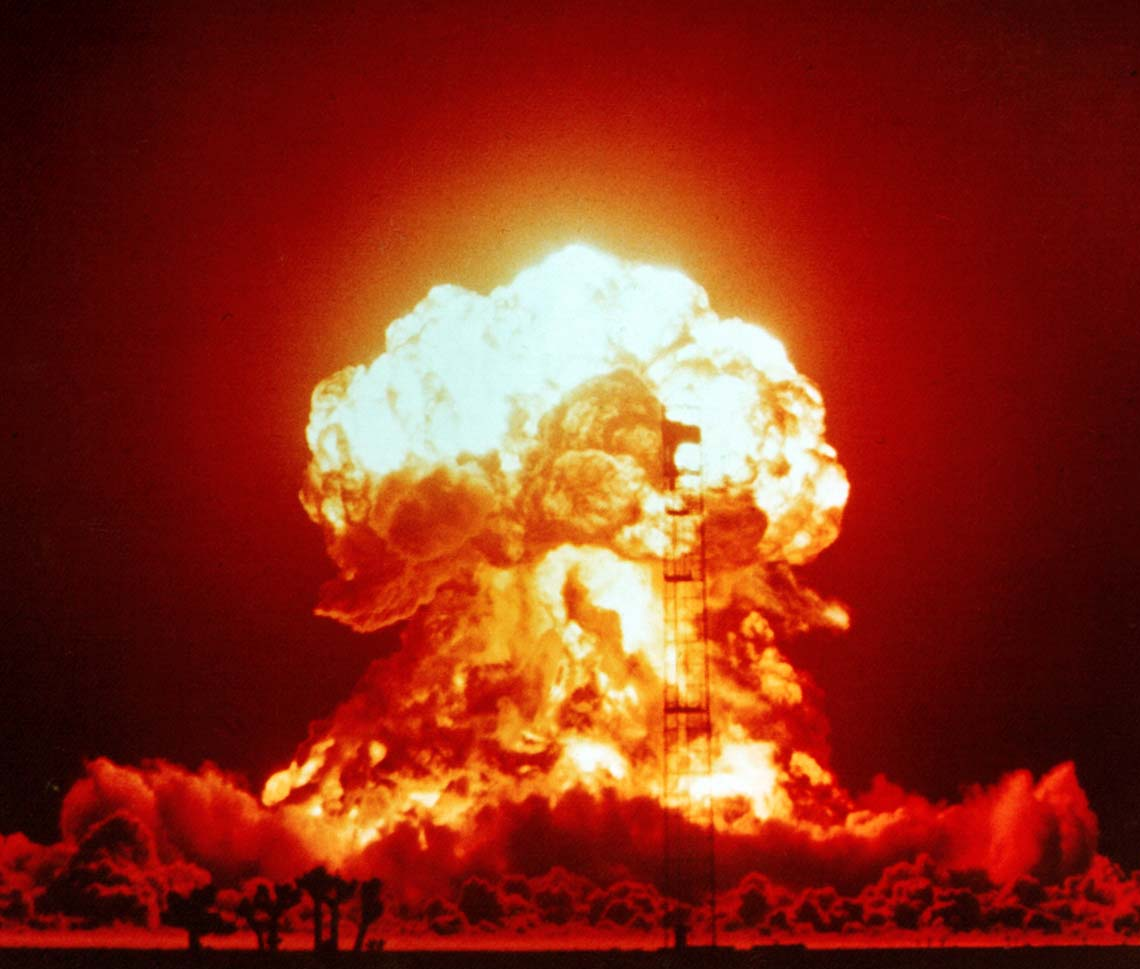
\includegraphics[width=\linewidth]{img/nuke.jpg}
		\end{figure}
	\end{column}
\end{columns}
\end{frame}

\begin{frame}{Infrasound Network}
\begin{figure}
	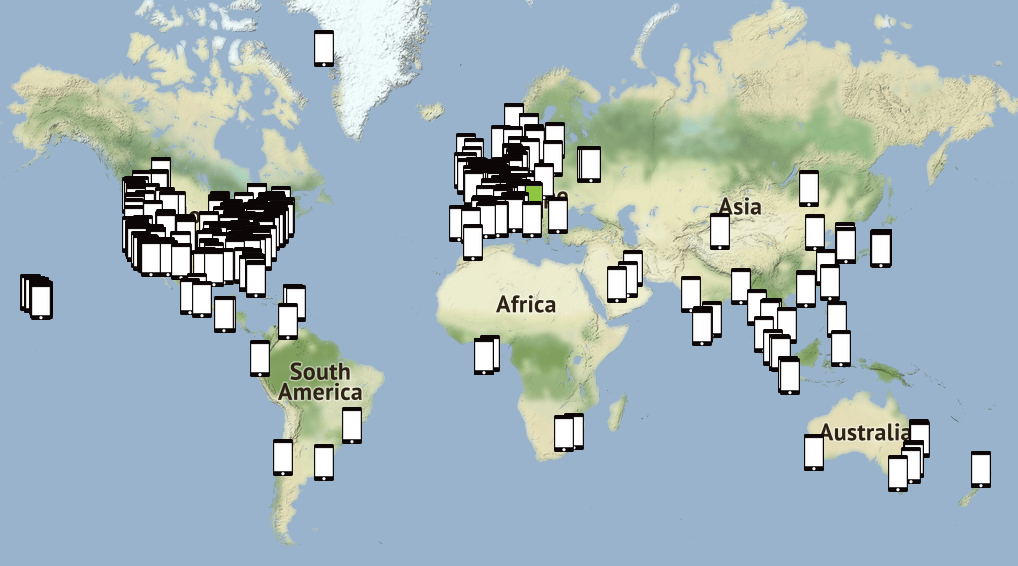
\includegraphics[width=\linewidth]{img/network.png}
\end{figure}
\end{frame}

\begin{frame}{National Labs}
\begin{itemize}
	\item Lawrence Livermore National Laboratory
	\begin{itemize}
		\item Internship
		\item National Ignition Facility
	\end{itemize}
	\item Idaho National Laboratory
	\begin{itemize}
		\item Got to tour a nuclear reactor
		\item Took measurements at Yellowstone National Park
	\end{itemize}
	\item Sandia National Laboratory
\end{itemize}
\end{frame}

\begin{frame}{Conferences}
\begin{columns}
	\begin{column}{.50\textwidth}
		\begin{itemize}
			\item Ann Arbor, Michigan
			\item Honolulu, Hawaii
			\item Minneapolis, Minnesota
			\item San Fransisco, California
			\item Raleigh, North Carolina 
		\end{itemize}
	\end{column}
	\begin{column}{.50\textwidth}
		\begin{figure}
			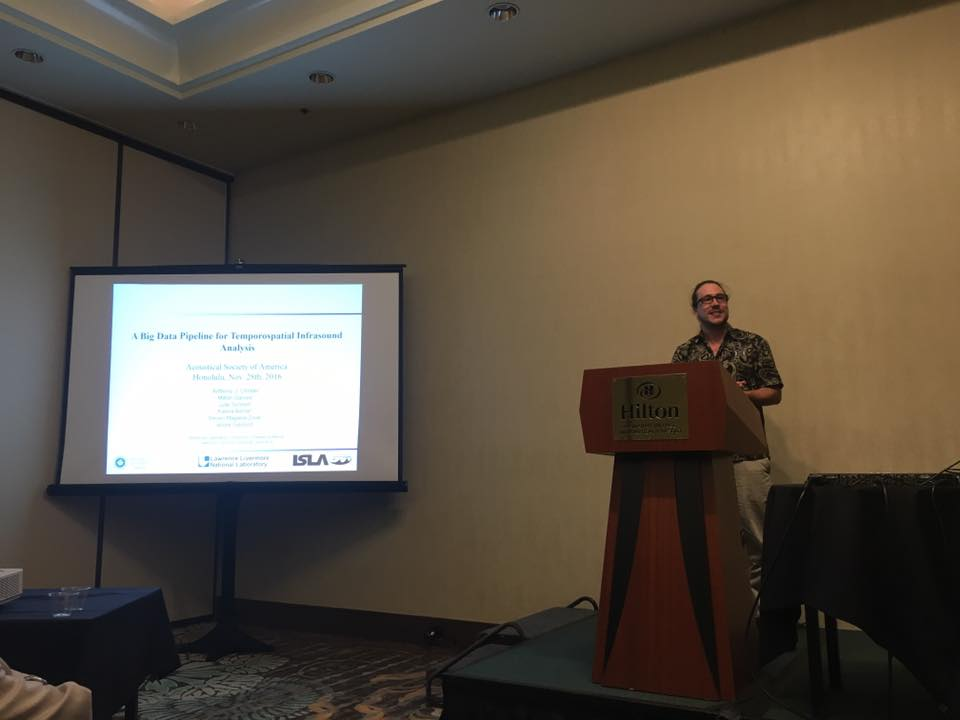
\includegraphics[width=\linewidth]{img/conference.jpg}
		\end{figure}
	\end{column}
\end{columns}
\end{frame}

\begin{frame}{Ph.D.}
\begin{itemize}
	\item Requires novel contribution to science
	\item General Ph.D. timeline
	\begin{itemize}
		\item Acceptance
		\item Qualifying Exam
		\item Portfolio
		\item \textbf{Proposal}
		\item Dissertation
		\item Defense
	\end{itemize}
\end{itemize}
\end{frame}

\section{Computer Science}
\begin{frame}{Is Computer Science Right for You?}
\begin{itemize}
	\item Strong communication skills?
	\item Enjoy working in a team?
	\item Want to work in multiple disciplines?
	\item Like solving puzzles?
	\item Mathematically minded?
	\item Enjoy learning?
\end{itemize}
\end{frame}

\begin{frame}{Computer Science is Broad}
\begin{itemize}
	\item Computer science is a broad subject consisting of many and varied subfields....
	\item Computer science is
	\begin{itemize}
		\item Theory
		\item Application
		\item Art
	\end{itemize}
\end{itemize}
\end{frame}

\begin{frame}{App Design}
\begin{itemize}
	\item iOS, Android development
\end{itemize}
\end{frame}

\begin{frame}{Artificial Intelligence (AI)}
\begin{itemize}
	\item Teaching computers how to learn
	\item Automatically recognizing patterns in images, sounds, data sets
	\item Deep learning / Neural networks
	\item Autonomous robots
\end{itemize}
\end{frame}

\begin{frame}{Computer Architecture}
\begin{itemize}
	\item Hardware design
	\item Processor design
	\item Microcontrollers
	\item Electronics
\end{itemize}
\end{frame}

\begin{frame}{Compiler Design}
\begin{itemize}
	\item Turn computer code into 1's and 0's that computer hardware understands
\end{itemize}
\end{frame}

\begin{frame}{Computer Graphics and Visualization}
\begin{itemize}
	\item Design plots and other visualiazations for large data sets
	\item Virtual Reality / Augmented Reality
	\item Video games
\end{itemize}
\end{frame}

\begin{frame}{Computer Networks}
\begin{itemize}
	\item How computers communicate with each other
	\item Secure communications
	\item Distributed sensor networks / mobile networks
\end{itemize}
\end{frame}

\begin{frame}{Computer Security}
	\begin{itemize}
		\item Both theoretical and practical
		\item Penetration testing
		\item Security protocols
		\item Bug hunting
		\item Best practices`
	\end{itemize}
\end{frame}


\begin{frame}{Computer Science Fields II}
\begin{itemize}
	\item Cryptography
	\item Databases
	\item Data Science
	\item Data Structures and Algorithms
	\item Distributed Systems
	\item Formal Methods
	\item Game design
\end{itemize}
\end{frame}

\begin{frame}{Computer Science Fields III}
\begin{itemize}
	\item High Performance Computing
	\item Human Computer Interaction (HCI)
	\item Image Processing

	\item Operating Systems
	\item Programming Languages
	\item Robotics
	\item Simulation Modeling
	\item Software Engineering
	\item Theory of Computation
\end{itemize}
\end{frame}

\begin{frame}{Thank You!}
\begin{columns}
	\begin{column}{.35\textwidth}
		Anthony Christe \\
		achriste@hawaii.edu
	\end{column}
	\begin{column}{.65\textwidth}
		\begin{figure}
			
\includegraphics[width=\linewidth]{img/meme.png}
		\end{figure}
	\end{column}
\end{columns}
\end{frame}

\end{document}
